\chapter{Построение математической модели}
\section{Постановка задачи}
Цель работы:
\begin{itemize}
	\item Сформулировать модель движения материальной точки во вращающейся системе координат.
	\item Проанализировать полученную модель
	\item Провести численные эксперименты с различными параметрами, для понимания влияния на траекторию движения.
\end{itemize}

Дано:
\begin{itemize}
	\item $\overrightarrow{r}$ - радиус-вектор, проведенный от центра вращения к материальной точке.
	\item $\overrightarrow{v'} = (u,v)$ - относительная скорость материальной точки ($[u] = [v]=$м/c).
	\item $\phi$ - широта на поверхности Земли (град.).
	\item $\omega$ - постоянная уголовая скорость поверхности (рад/с).
	\item $m$ - масса материальной точки (кг).
\end{itemize}
\section{Формализация}
Для вывода математической модели будем использовать полярную систему координат, второй закон Ньютона в дифференциальной форме и кориолисову силу в общей форме.

Пусть сила трения принебрежима мала, но диск/Земля передаёт своё вращение на материальную точку без изменения.
\newpage
\section{Построение модели}
\begin{figure}[h]  % Окружение для картинки
	\centering
	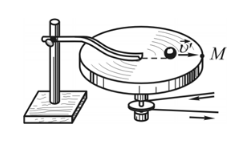
\includegraphics[height=0.2\textwidth]{imgs/base.png}  % Вставка изображения
	\caption{Движение на покоящейся поверхности.}  % Подпись к изображению
	\label{fig:base}  % Метка для ссылки
\end{figure}

Если тело движется относительно вращающейся системы отсчета, то на него
помимо центробежной силы инерции, действует еще одна сила инерции, которая
зависит от относительной скорости движения тела $\vec{v}$, и от угловой скорости $\vec{\omega}$ вращения системы отсчета. Этот вид инерции открыл Гаспар Кориолис. Соответственно силу называют \textit{кориолисовой}.

Для выяснения причин, которые вызывают возникновение силы Кориолиса, рассмотрим следующий опыт. Скатим с желоба шарик на центр диска, который может вращаться вокруг вертикальной оси. Таким образом, после
скатывания с желоба шарик будет двигаться по радиусу
неподвижного диска с постоянной скоростью $\vec{v}'$ в направлении точки $M$. 

\begin{figure}[h]  % Окружение для картинки
	\centering
	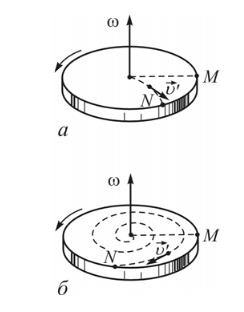
\includegraphics[height=0.4\textwidth]{imgs/rotation.png}  % Вставка изображения
	\caption{Движение на вращающейся поверхности.}  % Подпись к изображению
	\label{fig:rotation}  % Метка для ссылки
\end{figure}


Если диск привести в движение, то шарик отклонится от первоначальной траектории и придёт в точку $N$ (Рис. \ref{fig:rotation}, a). Причём, при небольшой относительной скорости шарика $\vec{v}'$ диск повернётся на больший угол и может совершить несколько оборотов (Рис. \ref{fig:rotation}, б).

\begin{figure}[h]  % Окружение для картинки
	\centering
	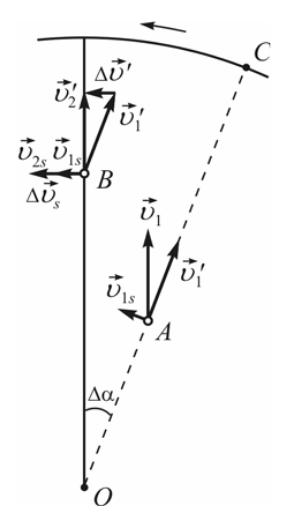
\includegraphics[height=0.6\textwidth]{imgs/velocity.png}  % Вставка изображения
	\caption{Проекции скоростей на вращающейся поверхности.}  % Подпись к изображению
	\label{fig:velocity}  % Метка для ссылки
\end{figure}

Рассмотрим эксперимент более подробно. 
Пусть шарик двигается равномерно из точки $A$ радиуса $OC$ со скоростью относительной $\vec{v}'$. 
Угловая скорость вращения диска равна $\vec{\omega} $ (направление вращение показано на рис. \ref{fig:velocity} стрелкой). 
За интервал $\Delta t$ шарик переместился на расстояние $\Delta l = \vec{v}' \Delta t $. 
За это же время в неподвижной системе координат радиус $OC$ повернётся на угол $\Delta \alpha = \omega \Delta t$, что перенесет шарик в точку $B$. 
В этой точке шарик будет иметь скорость, относительно неподвижной системы отчёта $\vec{v}$ (абсолютная скорость), которая складывается из $\vec{v}'$  и  переносной скорости $\vec{v}_s = [\vec{\omega} \times \vec{r}]$:
\begin{equation}
	\vec{v} = \vec{v}' + \vec{v}_s
	\label{eq:velocity}
\end{equation}
Распишем подробнее переносную скорость:
\[
\vec{v}_s = [\vec{\omega} \times \vec{r}] = \begin{vmatrix}
	\mathbf{i} & \mathbf{j} & \mathbf{k} \\
	0 & 0 & \omega \\
	x & y &  0
\end{vmatrix}
\]
Теперь вычислим определитель:

\[
\vec{v}_s = \mathbf{i} \begin{vmatrix}
	0 & \omega \\
	y & 0
\end{vmatrix} - \mathbf{j} \begin{vmatrix}
	0 & \omega \\
	x & 0
\end{vmatrix} + \mathbf{k} \begin{vmatrix}
	0 & 0 \\
	x & y
\end{vmatrix}
\]
Вычисляя каждый из определителей, получаем:

\[
\vec{v}_s = \mathbf{i} (0 - \omega y) - \mathbf{j} (0 - \omega x) + \mathbf{k} (0 - 0)
\]
Таким образом, результат будет:

\[
\vec{v}_s = -\omega y \mathbf{i} + \omega x \mathbf{j}
\]

Таким образом, при равномерном движении вдоль радиуса в неподвижной системе отсчёта будет существовать не только переносное ускорение 
\[
\vec{a_s} = -\omega^2 \vec{r},
\]
которое вызывает изменение направления скорости \(\vec{v_s}\), но и нормальное к радиусу ускорение \(\vec{a_k}\), вызывающее изменение направления скорости \(\vec{v'}\) и модуля скорости \(\vec{v_s}\).

Чтобы определить модуль этого ускорения, найдём указанные изменения скоростей за некоторый малый интервал времени \(\Delta t\). На рис. \ref{fig:velocity} изображены векторы относительных и переносных скоростей для двух положений шарика в точках \(A\) и \(B\), а также их изменения за рассматриваемый интервал времени \(\Delta \vec{v_s}\) и \(\Delta \vec{v'}\).

Поскольку нас интересует изменение только модуля вектора скорости в этих положениях, а не его направления, перенесём \(\vec{v_s}\) из положения \(A\) в положение \(B\) и направим вдоль вектора \(\vec{v_s}\). Получим отрезок \(\Delta v_s\), характеризующий изменение модуля скорости. Сумма модулей векторов \(\Delta \vec{v_s}\) и \(\Delta \vec{v'}\) будет представлять собой полное изменение абсолютной скорости в направлении, перпендикулярном радиусу за время \(\Delta t\), то есть ускорение движения шарика.

Если за время \(\Delta t\) радиус повернулся на угол \(\Delta \alpha = \omega \Delta t\), то 
\[
\Delta v' = v' \Delta \alpha = v' \omega \Delta t.
\]
За это же время шарик вдоль радиуса переместился на расстояние \(\Delta r = v' \Delta t\) и при этом скорость \(v_s = \omega r\) возросла по величине на 
\[
\Delta v_s = \omega \Delta r = \omega v' \Delta t.
\]
Как видно, оба эти изменения скорости равны по величине и имеют одинаковое направление. Поэтому полное изменение скорости в направлении, перпендикулярном радиусу, 
\[
\Delta v' + \Delta v_s = 2 v' \omega \Delta t.
\]
Следовательно, ускорение 
\[
a_k = \lim_{\Delta t \to 0} \frac{\Delta v' + \Delta v_s}{\Delta t} = 2 \omega v'.
\]

Это ускорение, зависящее как от относительной скорости \(v'\), так и от переносной скорости вращения \(\omega\), называется \textit{кориолисовым ускорением}. 
Направление этого ускорения всегда перпендикулярно к относительной скорости $\vec{v}'$. 

Очевидно, что при изменении направления вращения (\(\vec{\omega}\)) направление кориолисова ускорения \(\vec{a}_k\) изменится на противоположное. Аналогичный результат наблюдается и при изменении направления относительной скорости \(\vec{v'}\). Во всех случаях направление \(\vec{a}_k\) определяется по правилу правого винта.

Исходя из этих рассуждений, можно сделать вывод, что кориолисово ускорение \(\vec{a}_k\) выражается через удвоенное векторное произведение угловой скорости \(\vec{\omega}\) и относительной скорости \(\vec{v'}\):

\[
\vec{a}_k = 2 [\vec{\omega}, \vec{v'}].
\]


Таким образом, в результате анализа эксперимента установлено, что в неподвижной системе отсчёта шарик движется с абсолютным ускорением, которое является векторной суммой переносного ускорения \(\vec{a}_s\) и кориолисова ускорения \(\vec{a}_k\):

\[
\vec{a} = \vec{a}_s + \vec{a}_k = -\omega^2 \vec{r} + 2 [\vec{\omega}, \vec{v'}].
\]

Рассматривая движения шарика относителя наблюдателя, находящегося на диске, можно обнаружить, что возникает кориолисова сила 
\begin{equation}
	\vec{F}_k = 2m[\vec{v}, \vec{\omega}.]
\end{equation}
Отметим, что силу кориолиса вызывает обратное кориолисово ускорение:
\[
	\vec{a} = -2[\vec{\omega}, \vec{v}'] = 2[\vec{v}, \vec{\omega}],
\]
- которое появляется при переходе от неподвижной к
вращающейся системе отсчета.

\begin{figure}[h]  % Окружение для картинки
	\centering
	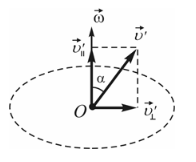
\includegraphics[height=0.3\textwidth]{imgs/earth.png}  % Вставка изображения
	\caption{Движение под углом к оси вращающения}  % Подпись к изображению
	\label{fig:earth}  % Метка для ссылки
\end{figure}

В общем случае тело может двигаться с относительной скоростью,
направленной под произвольным углом $\alpha$ к оси вращения (рис. \ref{fig:earth}). Разложим
вектор скорости  $\vec{v}' $на две составляющие: $\vec{v}'_\perp$, которая лежит в плоскости,
перпендикулярной оси вращения, и $\vec{v}'_{\parallel}$, параллельную оси вращения.
Составляющая $\vec{v}'_{\parallel}$ не изменяет переносной скорости тела, потому что угол между$\vec{v}'_{\parallel}$ и $\vec{\omega}$ равен нулю. Поэтому сила Кориолиса обусловлена лишь составляющей $\vec{v}'_\perp = \vec{v}'\sin(\alpha)$ .

Таким образом мы получили дифференциальное уравнение второго порядка для движения на вращающейся системе координат:

\begin{equation}
	\frac{d^2\vec{r}}{dt^2} = 2\left[\frac{d\vec{r}}{dt}, \vec{\omega}\right]\sin(\phi)
	\label{eq:difr}
\end{equation}

Чтобы перейти к дифференциальным уравнениям движения по координатам $x$ и $y$, нужно разложить ускорение (\ref{eq:difr}) по декартовым осям:
\begin{equation}
	\begin{cases}
		\ddot{x} = 2\omega \dot{y} \sin(\phi),\\
		\ddot{y} = - 2\omega \dot{x}\sin(\phi).
	\end{cases}
\end{equation}
 
 Получили дифференциальное уравнение второго порядка. Следовательно для нахождения единственного решения следует ввести начальные координаты материальной точки и её относительную скорость по каждой из координат:
 \[
 	\begin{cases}
 		x(0) = x_{0}, & \dot{x}(0) = x_{1} \\
 		y(0) = y_{0}, & \dot{y}(0) = y_{1}
 	\end{cases}
 \]
